\documentclass[12pt,letterpaper]{article}
\usepackage[utf8]{inputenc}
\usepackage[spanish]{babel}
\usepackage{amsmath}
\usepackage{amsfonts}
\usepackage{amssymb}
\usepackage{float}
\usepackage{graphicx}
\usepackage{listings}
\usepackage{float}
\usepackage{pdfpages}
\usepackage[left=3cm,right=3cm,top=4cm,bottom=3cm]{geometry}
\usepackage[usenames,dvipsnames]{color}
\lstset{ 
  language=R,
  basicstyle=\ttfamily,
  numbers=left,
  numberstyle=\color{Blue},
  stepnumber=1,
  numbersep=5pt,
  backgroundcolor=\color{white},
  showstringspaces=false,
  showtabs=false,
  frame=single,
  rulecolor=\color{black},
  tabsize=2,
  captionpos=b,
  breaklines=true,
  breakatwhitespace=false,        
  keywordstyle=\color{RoyalBlue},
  commentstyle=\color{YellowGreen},
  stringstyle=\color{ForestGreen}
}







\author{Liliana Saus \\ Práctica 10}
\title{Algoritmo Genético \\   \begin{large}
\end{large}}

\begin{document}
\maketitle

\section*{Introducción}
La práctica 9 es sobre el uso de  algoritmos; genético y exacto , en particular para el problema de la mochila, donde la tarea consiste en:
\begin{itemize}
\item Seleccionar un subconjunto de objetos de tal forma que no se exceda la capacidad de la mochila en términos de la suma de los pesos de los objetos incluidos.
\item El valor total de los objetos incluidos sea lo máximo posible
\end{itemize}
\section*{Objetivo} 
Se paraleliza el algoritmo genético y se estudia los efectos en su tiempo de ejecución con pruebas estadísticas y visualizaciones, variando el número de objetos en la instancia. Además se determina con qué tamaño de instancia el algoritmo genético es mejor que el algoritmo exacto en términos de valor total obtenido por segundo de ejecución.

\section*{Datos experimentales }
 Se realizó la simulación para intancias con  $n=50,100,200$ durante $50$ iteraciones y con $10$ réplicas. Se tomaron esa cantidad de réplicas por características de la computadora empleada. 
 Para poder llevar acabo el objetivo, en la versión paralela del algoritmo génetico se paralelizaron las fases:
 \begin{itemize}
\item Mutación
\item Reproducción 
\item Factibilidad
\item Objetivo
 

 \newpage
\section*{Resultados}
Se ejecutaron la versión secuencial y paralela, para comparar los tiempos, la figura 1 muestra  los resultados. Se ve que los tiempos de ejecución para la versión secuencial son más grandes que para la versión paralela. 

\begin{figure}[ht]
  \centering
  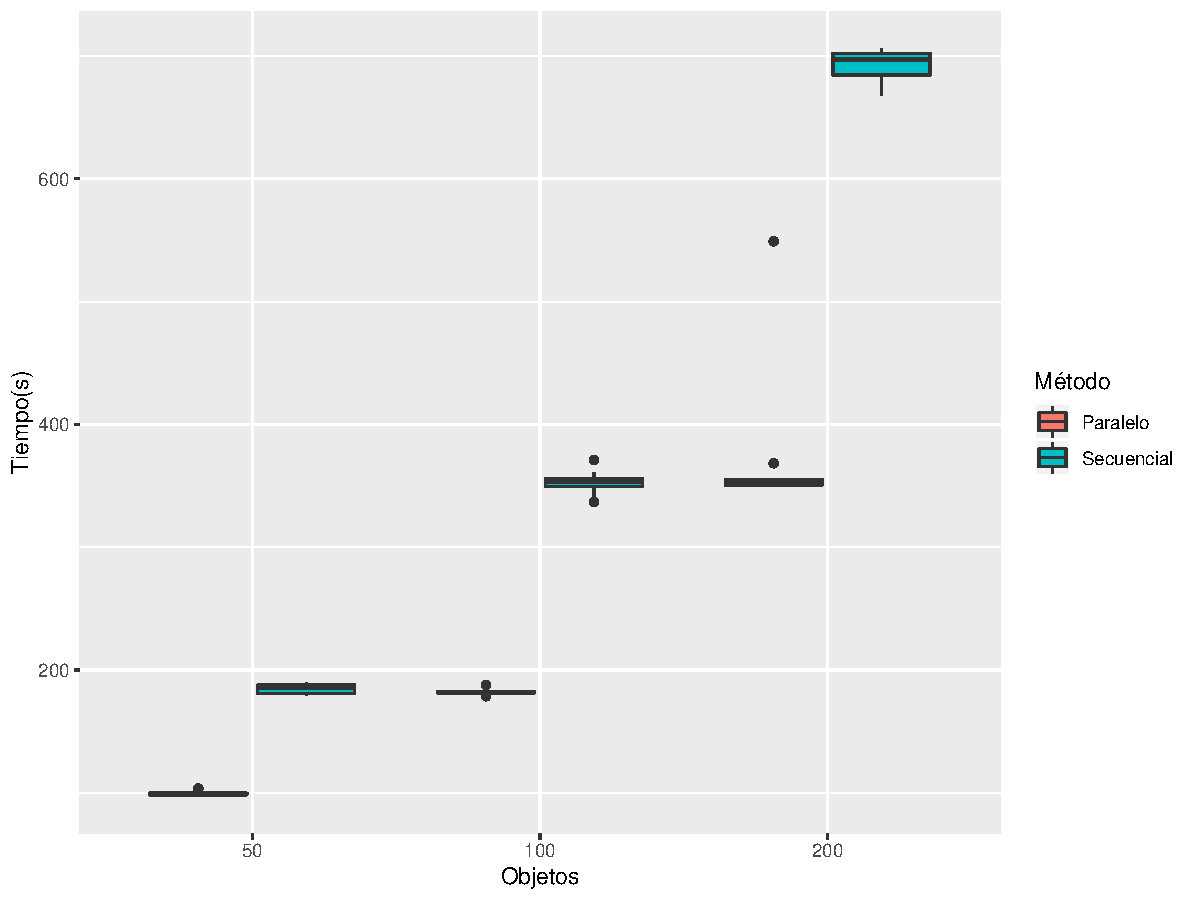
\includegraphics[scale=.8]{Rplot}
  \caption{Tiempo de ejecución paralela y secuencial.}
\end{figure}
\newpage
Se realiza la prueba de $Shapiro-Wilk$ para examinar si los datos cumplen con normalidad. 
\begin{lstlisting}
> Shapiro.test(resultados$tiempo)

    Shapiro-Wilk normality test

data:  resultados$Tiempo
W = 0.82121, p-value = 4.754e-07
\end{lstlisting}
Como el p-valor es menor que 0.05, se concluye que los datos no cumplen normalidad. Asi que se realiza una prueba estadística no paramétrica $Kruskal-Wallis$

\begin{lstlisting}
> kruskal.test(tiempo ~ Método, data = Resultados)

    Kruskal-Wallis rank sum test

data:  Tiempo by Método
Kruskal-Wallis chi-squared = 15.582, df = 1,
p-value = 7.899e-05
\end{lstlisting}
Como el p-valor es menor que 0.05 se rechaza la hipotesis nula, es decir que hay diferencias significativas en los tiempos. 

Por otro lado se calculo el beneficio entre el método exacto y el genético, usando 
\begin{equation}
\text{beneficio}= \frac{\text{objetivo}}{\text{suma total de los objetivos}}
\end{equation}

En la figura 2 se muestran los resultados, es fácil ver que hay un mayor beneficio en el algoritmo exacto que en el genético. 
\begin{figure}[H]
  \centering
  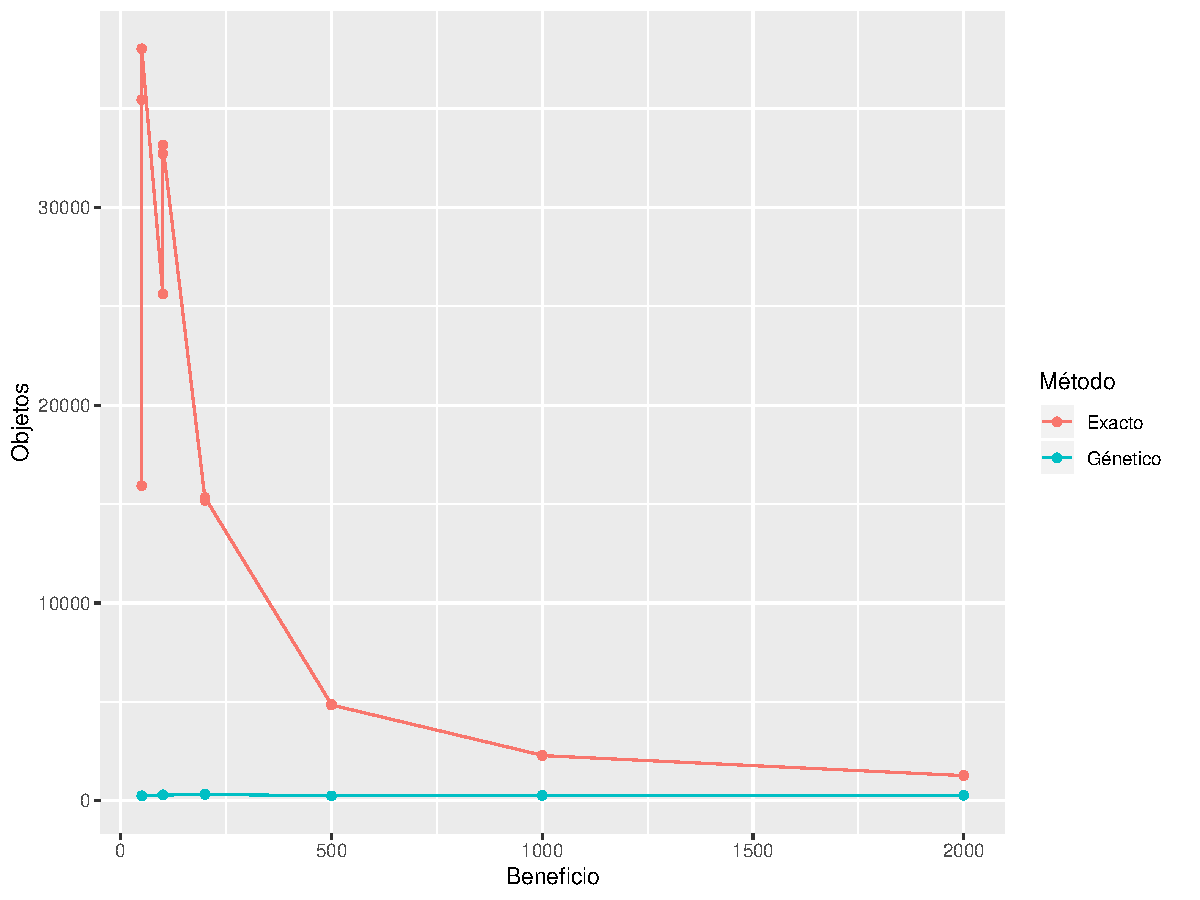
\includegraphics[scale=0.8]{tarea}
  \caption{Beneficio entre algoritmo genético y exacto.}
\end{figure}
Estos resultados podrían cambiar si se realiza un ajuste en los parámetros. 
\newpage
\section*{Reto 1}
El primer reto se cambia la selección de padres para reproducción a que use selección de ruleta: cada solución se selecciona como padre con una probabilidad que es proporcional a su valor de función objetivo y a su factibilidad, combinando los dos. Se estudia si este cambio produce una mejora estadísticamente significativa en la calidad de la solución. 


La figura 3 muestra la función objetivo aplicando el método con ruleta y sin ruleta, lo que se puede observa que se alcanza un mejor valor por el método sin ruleta. 

\begin{figure}[H]
  \centering
  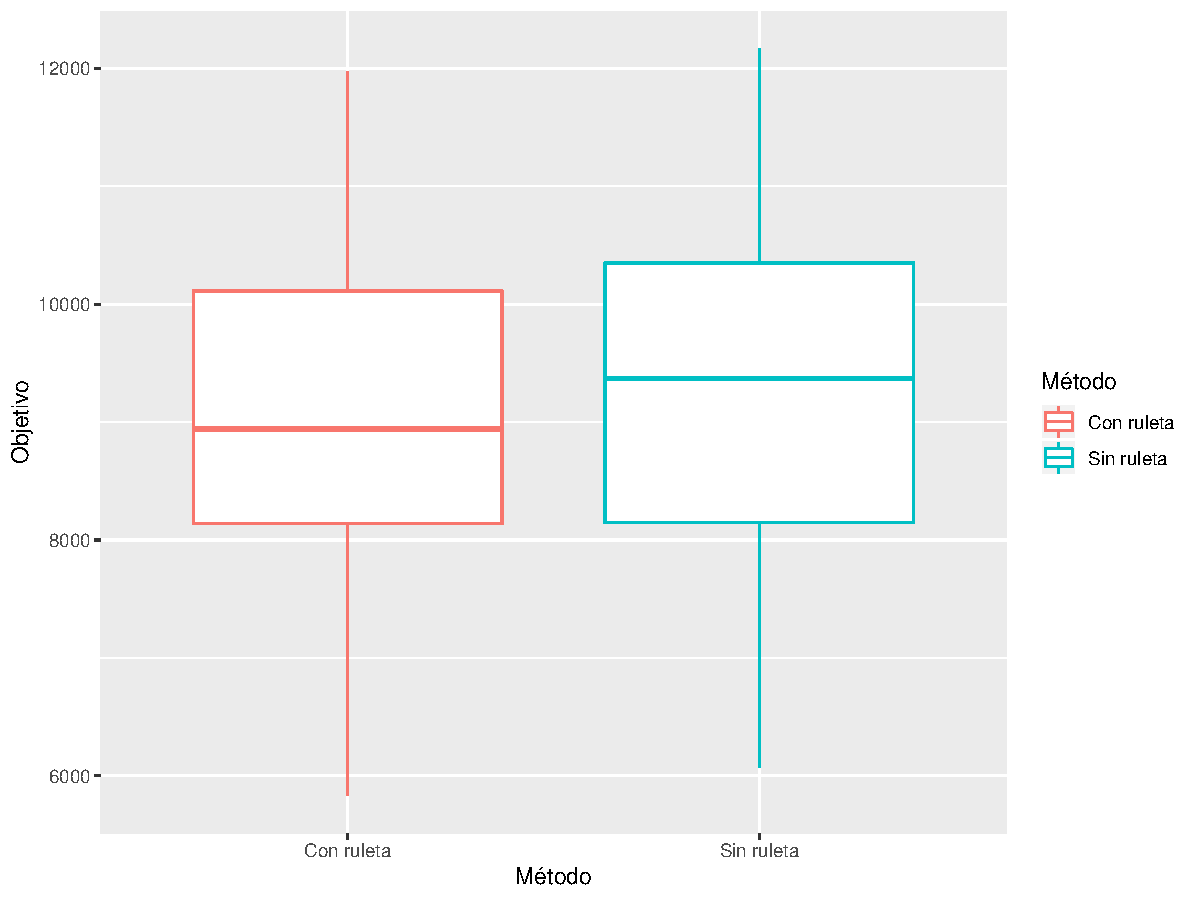
\includegraphics[scale=.8]{reto}
  \caption{Función objetivo con ruleta y sin ruleta }
\end{figure} 

Para probar si hay diferencia significativa entre los datos se realiza una prueba $Kruscal-Wallis$

\begin{lstlisting}
> kruskal.test(tiempo ~ Método, data = Resultados)

    Kruskal-Wallis rank sum test
data:  datos$Objetivo by Método
Kruskal-Wallis chi-squared = 0.41333, df = 1,
p-value = 0.5203

\end{lstlisting}
Como el p-valor es mayor que 0.05, aceptamos la hipótesis nula, por lo que se concluye que no hay nivel de significancia entre los datos. Se puede decir que haciendo un ajuste de parámetros se llegaría a otros resultados. 

\section*{Reto 2}
El segundo reto es extender la selección de ruleta a la fase de supervivencia: en vez de quedarse con las mejores soluciones, cada solución tiene una probablidad de entrar a la siguiente generación que es proporcional a su valor de la función objetivo, incorporando el sí o no es factible la solución en cuestión, permitiendo que los $k$ mejores entre las factibles entren siempre. Se estudia nuevamente el efecto de este cambio en la calidad de la solución.
La figura 4 muestra la función objetivo aplicando el método con ruleta y sin ruleta, lo que se puede observa que se alcanza un mejor valo por el método sin ruleta. 
\newpage
\begin{figure}[H]
  \centering
  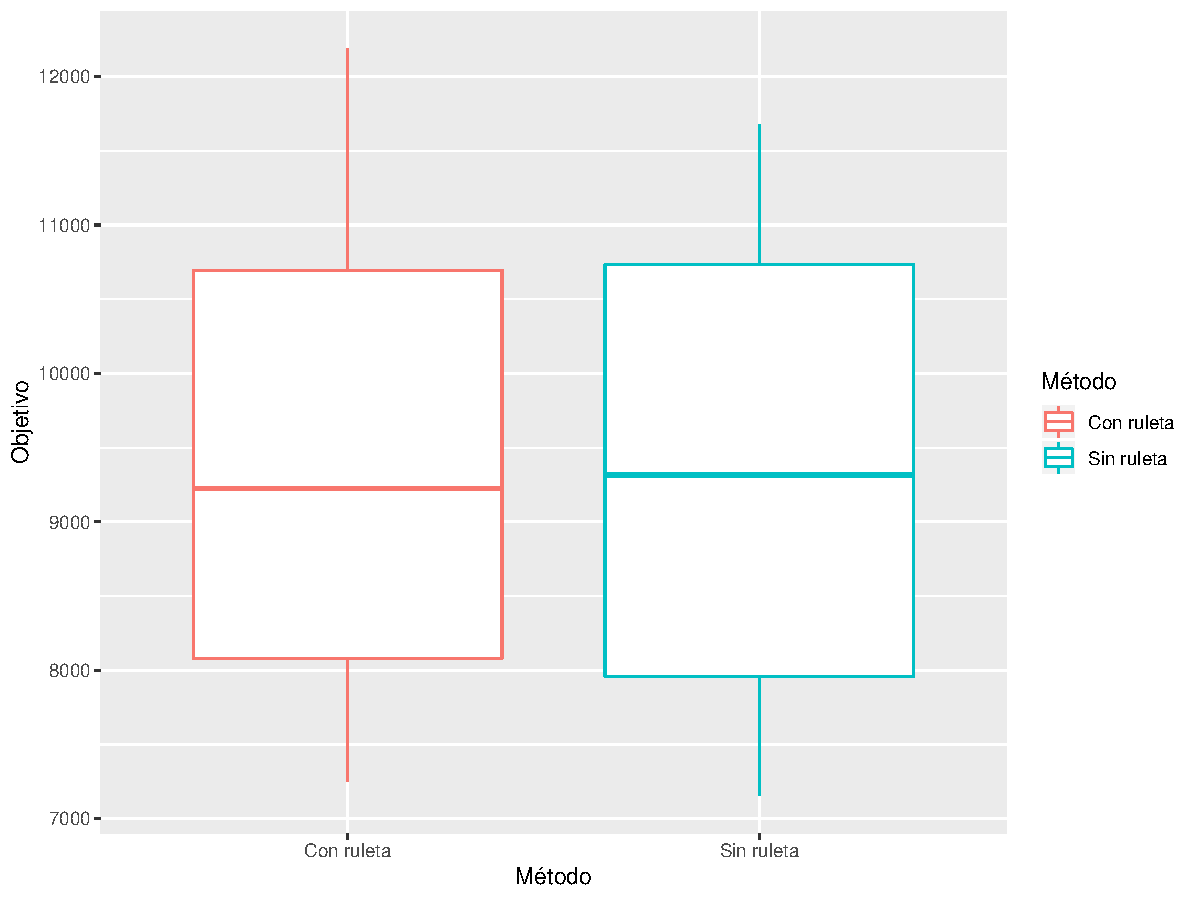
\includegraphics[scale=.8]{rreto2}
  \caption{Función objetivo con ruleta y sin ruleta }
\end{figure}
\newpage
Para probar si hay diferencia significativa entre los datos se realiza una prueba $Kruscal-Wallis$

\begin{lstlisting}
 kruskal.test(tiempo ~ Método, data = Resultados)

    Kruskal-Wallis rank sum test

data:  datos$Objetivo by Método
Kruskal-Wallis chi-squared = 0.03694, df = 1,
p-value = 0.8476
\end{lstlisting}
Como el p-valor es mayor que 0.05, aceptamos la hipótesis nula, por lo que se concluye que no hay nivel de significancia entre los datos.
Por lo que haciendo un ajuste de parámetros se podría llegar a otros resultados. 
\newpage
\begin{thebibliography}{X}
\bibitem{Zill2} \textsc{Elisa Schaeffer} \textit{R paralelo: simulación and análisis de datos, 2018.} \texttt{https://elisa.dyndns-web.com/teaching/comp/par/ }

\end{thebibliography}



\end{document}